\section{Vocabulario de Accidentes de Bicicletas}

Para el vocabulario asociado con los accidentes de bicicletas en el ayuntamiento de Madrid se ha elegido la siguiente fuente Datos.Madrid \cite{datosMadrid_accidentesDeBicicleta}.
En ella se muestran los accidentes de tráfico con implicación de bicicletas dentro de la jurisdicción del ayuntamiento.
\\
\\
La organización del conjunto de datos se hará siguiendo el diagrama \ref{fig:diagramaOntologAccid}

\begin{figure}[h]
	\centering
		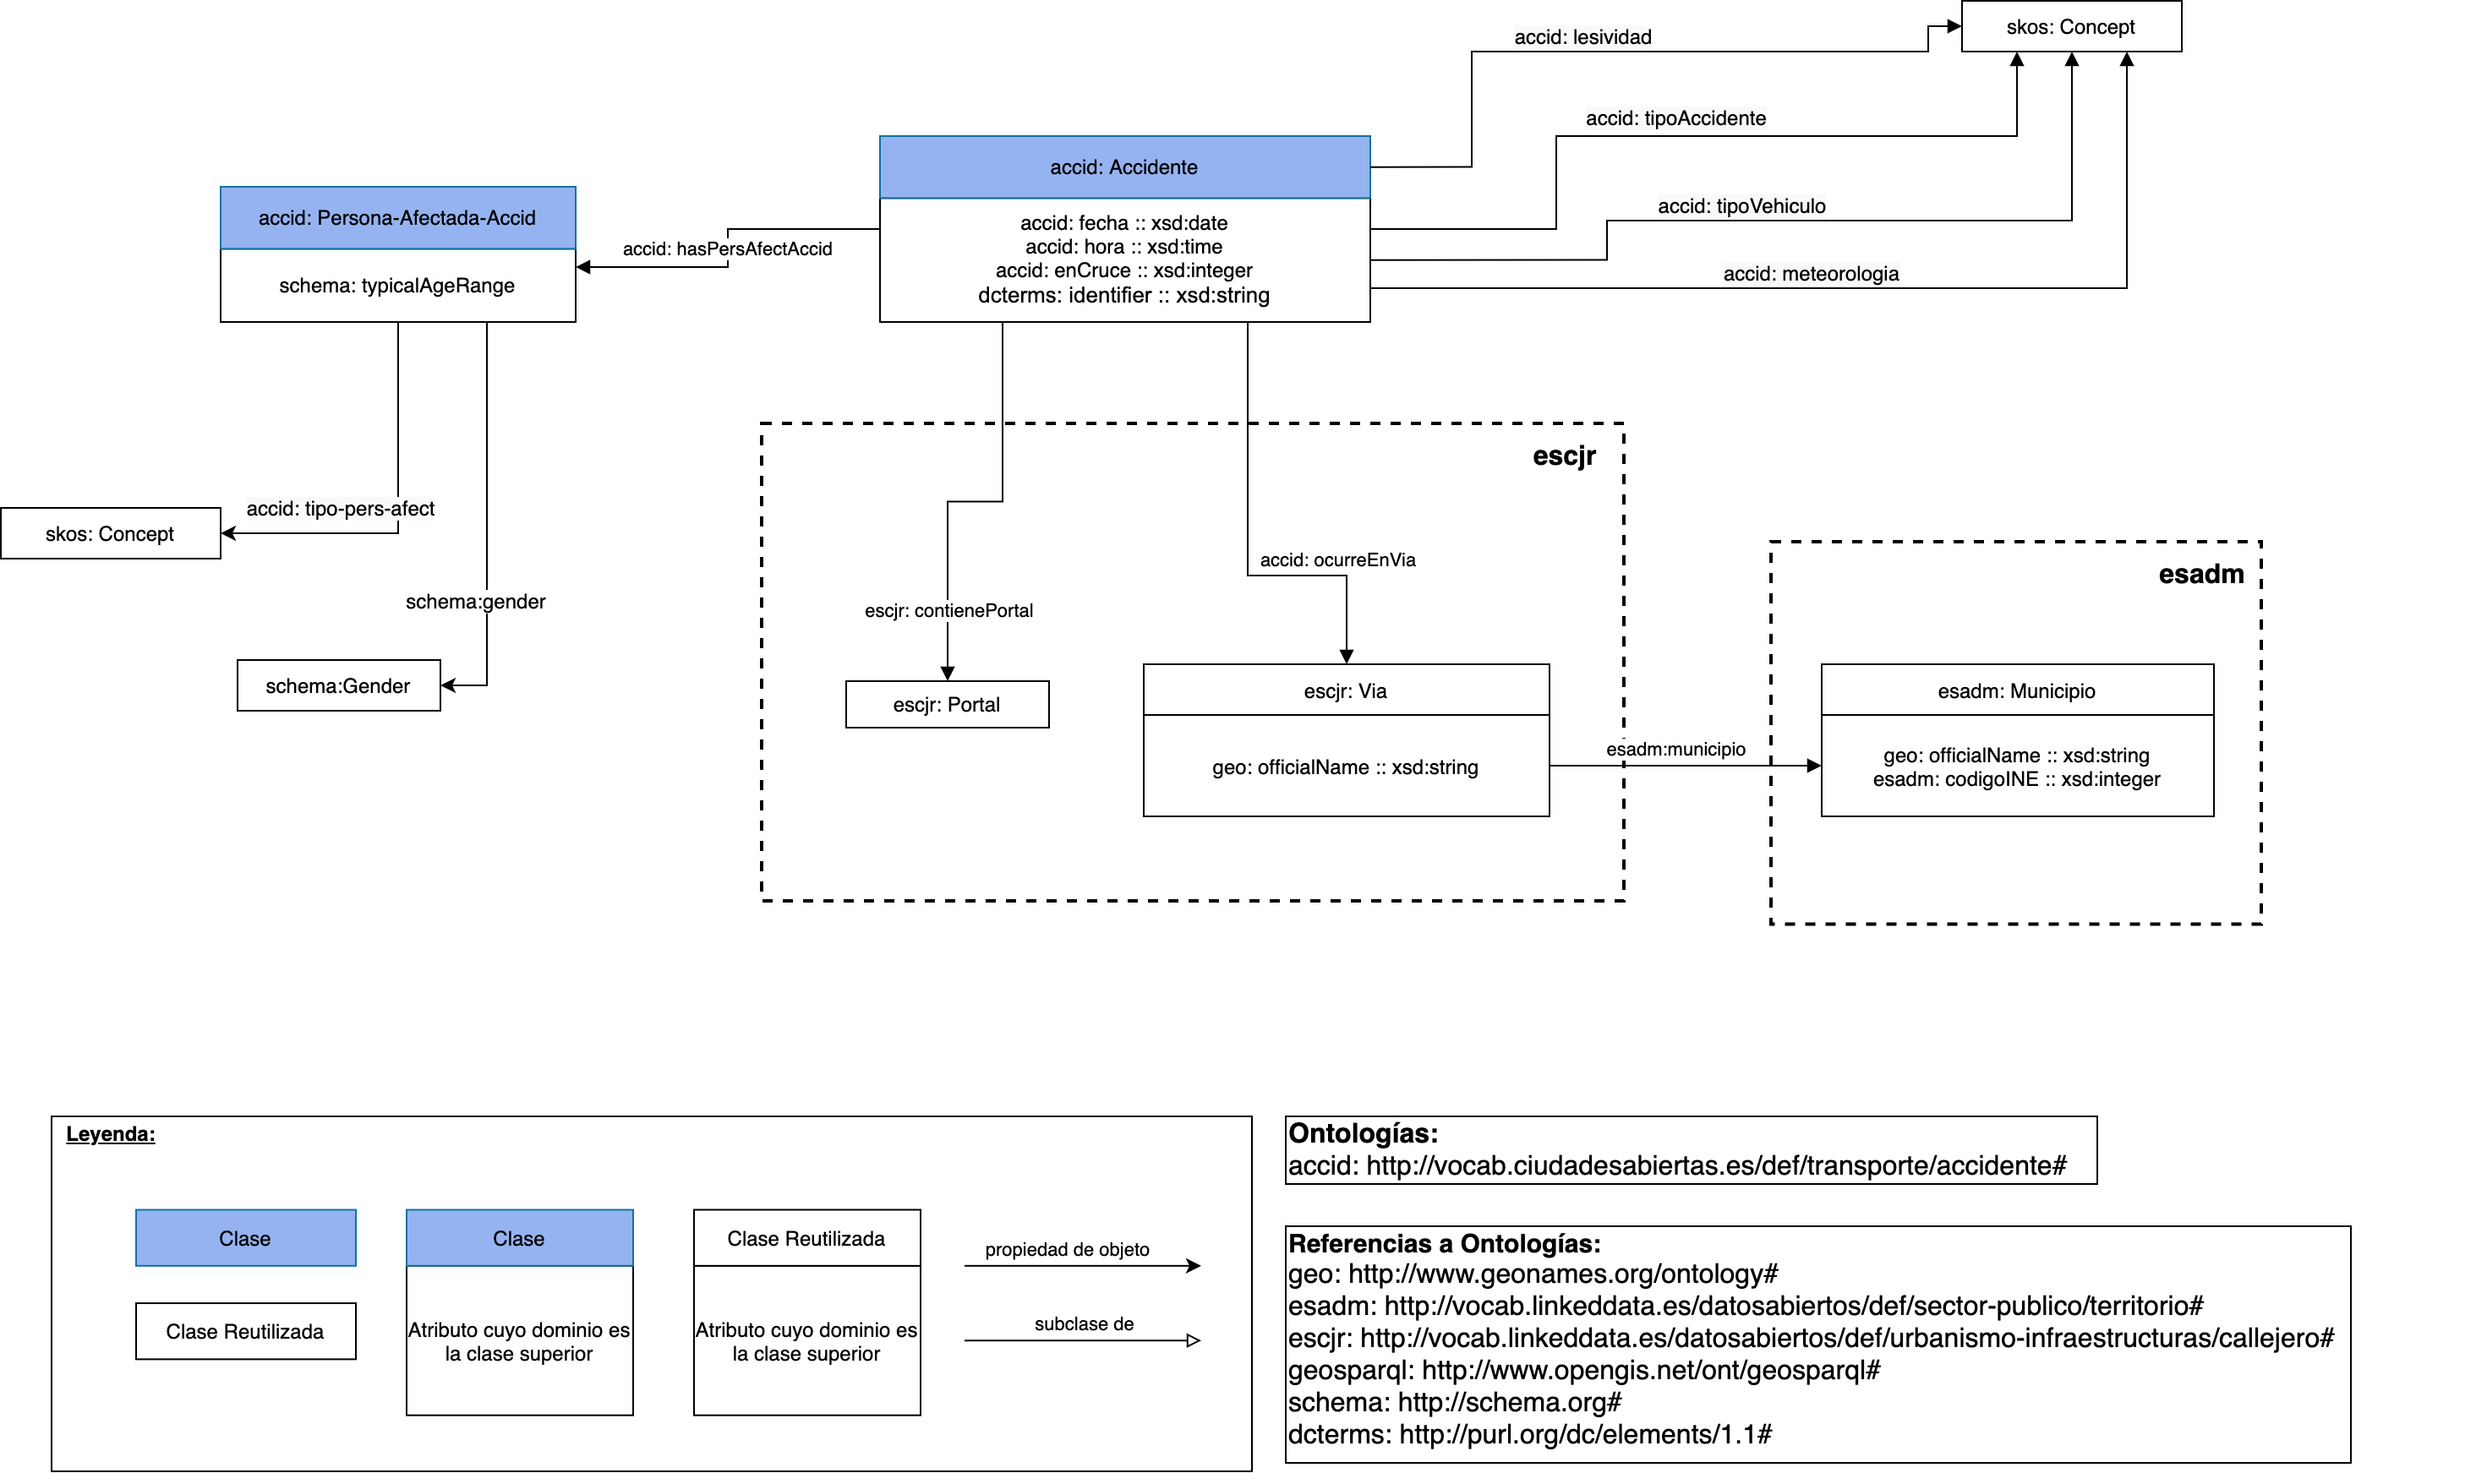
\includegraphics[angle=0, width=0.8\textwidth]{images/diagramaAccidBici.png}  
	\caption{Diagrama de Ontología de Accidentes con implicación de bicicletas en Madrid.}
	\label{fig:diagramaOntologAccid}
\end{figure}


Para la representación de los datos de accidentes de trafico con bicicletas se han definido varias clases y propiedades. Se han reutilizado elementos ya definidos en el vocabulario de Callejero \cite{ciudadesbiertas_callejero} y de Schema \cite{schema_org}.

\clearpage
En la siguiente tabla se muestran los Namespaces usados.

\begin{figure}[h]
	\centering
		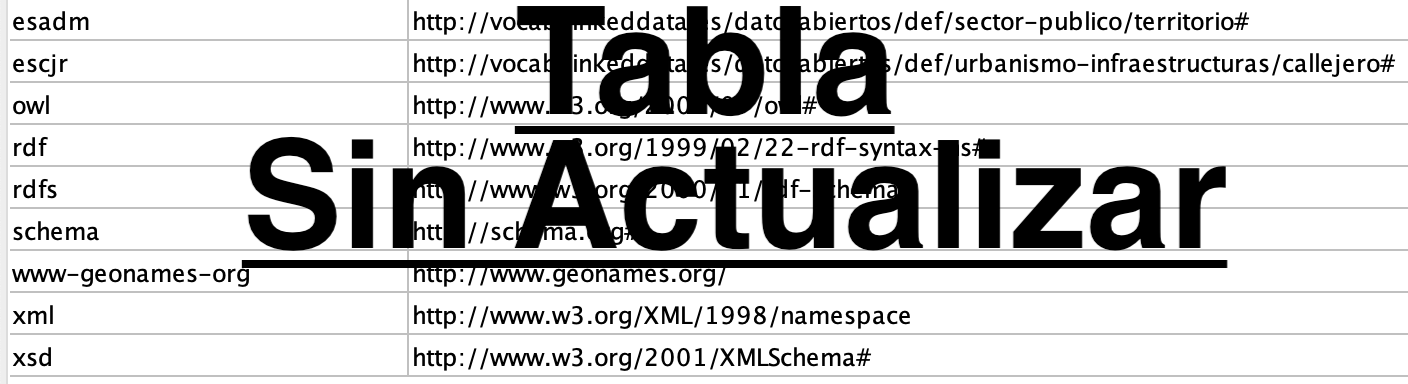
\includegraphics[angle=0, width=0.8\textwidth]{images/tablaIRIsAccidentesBici.png}  
	\caption{Namespaces usados para Accidentes de Bicicletas}
\end{figure}



Se ha optado por mantener la separación de elementos como fecha y hora, calle y numero debido a que la fuente de origen los tiene así dispuestos y en la posterior aplicación final que se va a construir será más conveniente tener esa información por separado, para poder disponer de datos a horas con menos luminosidad o calles completas(sin conocer la posición exacta), por ejemplo.


Para este conjunto de datos se ha optado por añadir, además de los ya proporcionados por la fuente de origen del ayuntamiento, nueva información como la propiedad "esCruce", el municipio, el tipo de via o el identificador de via. Son propiedades inferidas de la información proporcionada que permiten que sea más sencillo su tratamiento y uso, para esta u otras aplicaciones que puedan tener estos datos.
EsCruce se obtendrá del nombre de la calle, del cual atendiendo a varios patrones se puede determinar si el accidente ha ocurrido en una intersección de dos o más vías.
El Municipio se ha añadido para su posible reutilización posterior utilizando otros datasets de otras localidades, en este caso será siempre "Madrid".
El Tipo de Via de nuevo se obtendrá, a partir de los nombres de las calles, siguiendo unos patrones y palabras clave que determinen si es Calle, Avenida, Plaza... lo cual facilitará además su posterior cruce con otros datasets que también utilicen esta propiedad.
El Identificador de Via se obtendrá comparando el nombre de la via y su tipo con el Callejero de Madrid, el cual proporcionará este valor único que represente la via.

En este conjunto de datos se ha hecho un cambio importante con respecto al original y que será detallada en la sección Transformaciones en los vocabularios Fase1. Los accidentes que han ocurrido entre un cruce de vias se han separado en tantos registros como vias interfieran. De este modo será mucho más simple la búsqueda de accidentes ocurridos en una via y se podrá hacer una búsqueda más sencilla de ellas. Para no perder ninguna información el nombre del lugar donde ha ocurrido el accidente se conservará igual (es decir, con la descripción del cruce de vias) y se podrá identificar si dos o más registros pertenecen al mismo accidente por el número de expediente, el cual se conserva igual en ambos.



